%% LaTeX2e class for student theses
%% sections/content.tex
%% 
%% Karlsruhe Institute of Technology
%% Institute for Program Structures and Data Organization
%% Chair for Software Design and Quality (SDQ)
%%
%% Dr.-Ing. Erik Burger
%% burger@kit.edu
%%
%% Version 1.3, 2016-12-29

\chapter{Privacy Concept}
\label{ch:PrivacyConcept}

Many say: Data is the new oil and the most valuable resource there is. This shows us how important it is that we keep in control of our personal data. In order to achieve this, many players have to fulfill their obligations. On the one hand, the personal awareness of every user himself to only communicate the required and necessary information. On the other hand, the data handling institutes duty to guarantee legal compliance to laws like the EU’s general data protective regulations. While we can't act for the individual, we can provide tools and rules for institutions to help with legal compliance.

\section{General Concept}
\label{sec:PrivacyConcept:general}

The EU General Data Protective Regulations clearly states, that data of EU citizens have to be saved and processed inside EU countries \cite{personaldata.2011}. The only exception is a small set of countries with equal data protective laws. As a consequence, we need a simple data-flow analysis (\autoref{sec:RelatedWork:dataflow}) to know the data distribution in our software system. Frankly speaking, we must know which data is where in our system. This task got especially important, since distributed cloud system are a reality and data saved on "on premise" servers are becoming increasingly rare.

As mentioned in \autoref{sec:RelatedWork:dataflow}, the automated data-flow analysis on architecture level is still in its fledgling stages and therefore not suited for practice. As a compromise we decided on manual data tagging. To ease the data tagging and analysis process, we decided to use the common well defined categories \cite{Schmieders.2015}:
%A growing and continuous research field is exploring and developing approaches for automated data-flow analysis. However, these are still very limited and are therefore not yet suited for practice (see \autoref{sec:RelatedWork:dataflow}). Due to these limitations, we need manual annotation of components.

\begin{itemize}
	\item \textbf{Type 0: Personal Information}: Data stand in direct or indirect relation to personal information. This is independent from encryption or pseudonymization.
	
	\item \textbf{Type 1: Personally Identifiable Information}:  Data do not contain personal information. However, by combining, fusing or analysing data sets the personal data could be reconstructed for complete or partial personal information.
	
	\item \textbf{Type 2: Anonymous Data}: Data don't contain any personal information. Even by extensive data analysing no direct or indirect personal data can be extracted.
	
	\label{sec:PrivacyConcept:dataprivacylevel}
\end{itemize}

We use three categories, because in many cases data don't contain any direct or indirect link onto private data, however still contain indicators onto private data. For example an online shop wants to analyse, which products usually get ordered together. The orders get anonymized by removing the customer and the shipping address. Nevertheless, the time-stamp is required to get a timed evaluation factor. This data are not personal. However, combining and evaluating these with user-login-times, also non-personal data, privacy relevant data can be extracted. This also disqualifies them for Type 2, completely anonymous data. \cite{Schmieders.}\cite{Schmieders.2015}

To summarize, we use a manual, categorized annotation approach to identify a system components privacy level. Based on this privacy level we can check, whether a system deployment is privacy compliant.


\section{Deployment Constraints}
\label{sec:PrivacyConcept:deploymentrules}

How can we guarantee legal compliant distribution? As mentioned in \autoref{sec:Introduction:motivation}, personal data of EU citizens are only allowed to be processed, transferred or saved inside EU countries [...]. We argue that the following constraints, combined with correct manual annotation, are sufficient to accomplish this:

\begin{itemize}
	\label{enum:deployment_rules}
	\setlength\itemsep{0em}
	\item \textbf{Rule \#1}: Type 0 components must be deployed in a "save" geo-location.
	\item \textbf{Rule \#2}: Type 2 components can be deployed anywhere.
	\item \textbf{Rule \#3}: Type 1 components can be deployed anywhere.
	\item \textbf{Rule \#4}: Only deploy Type 1 components together in an "un-save" geo-location, if they receive their information (transitively) from the same Type 1 component.
\end{itemize}



\begin{wrapfigure}{l}{0.55\textwidth}
	\begin{center}
		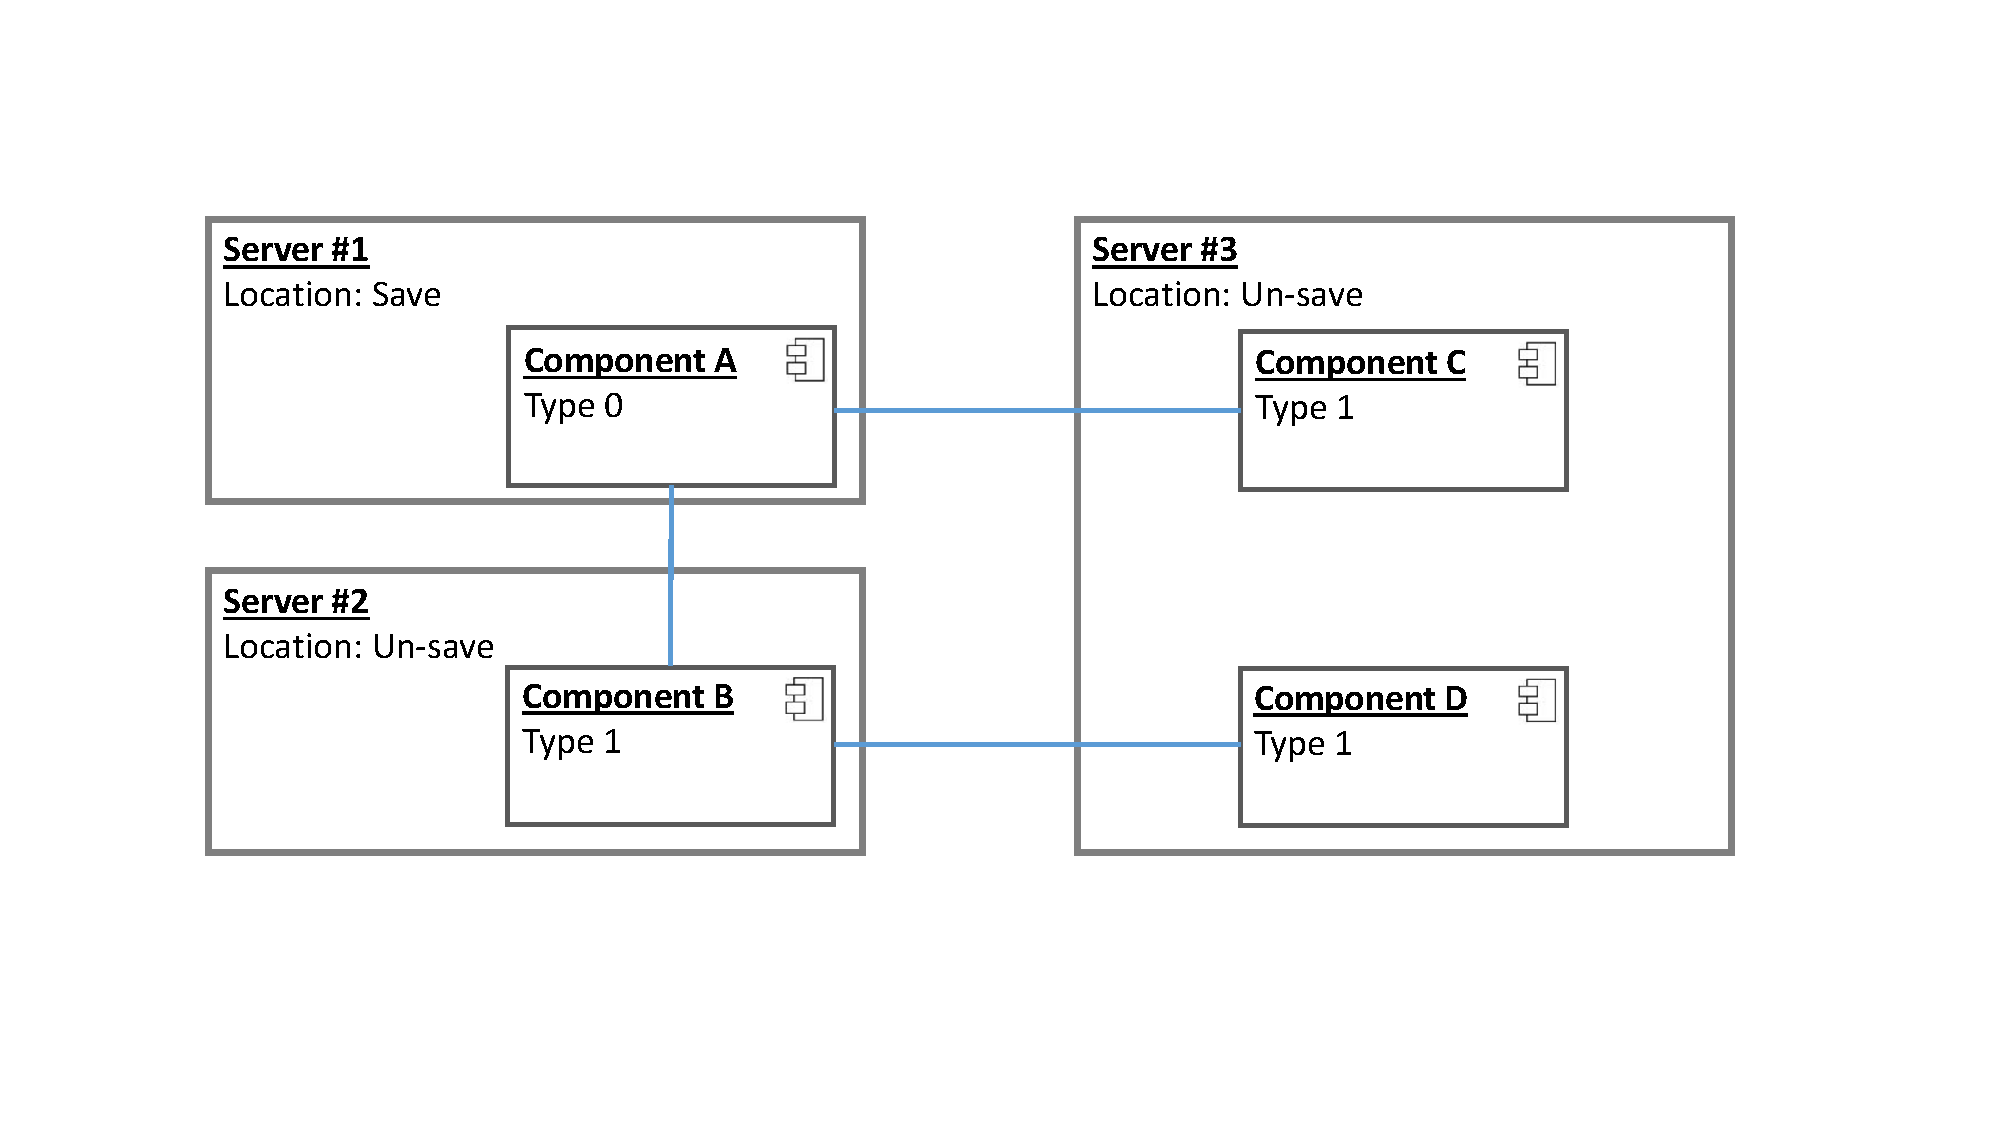
\includegraphics[trim = 35mm 45mm 40mm 30mm, clip, width=0.53\textwidth]{graphs/deployment_example_1}
	\end{center}
	\caption{Privacy violating deployment}
	\label{fig:example_depl:1}
	\begin{center}
		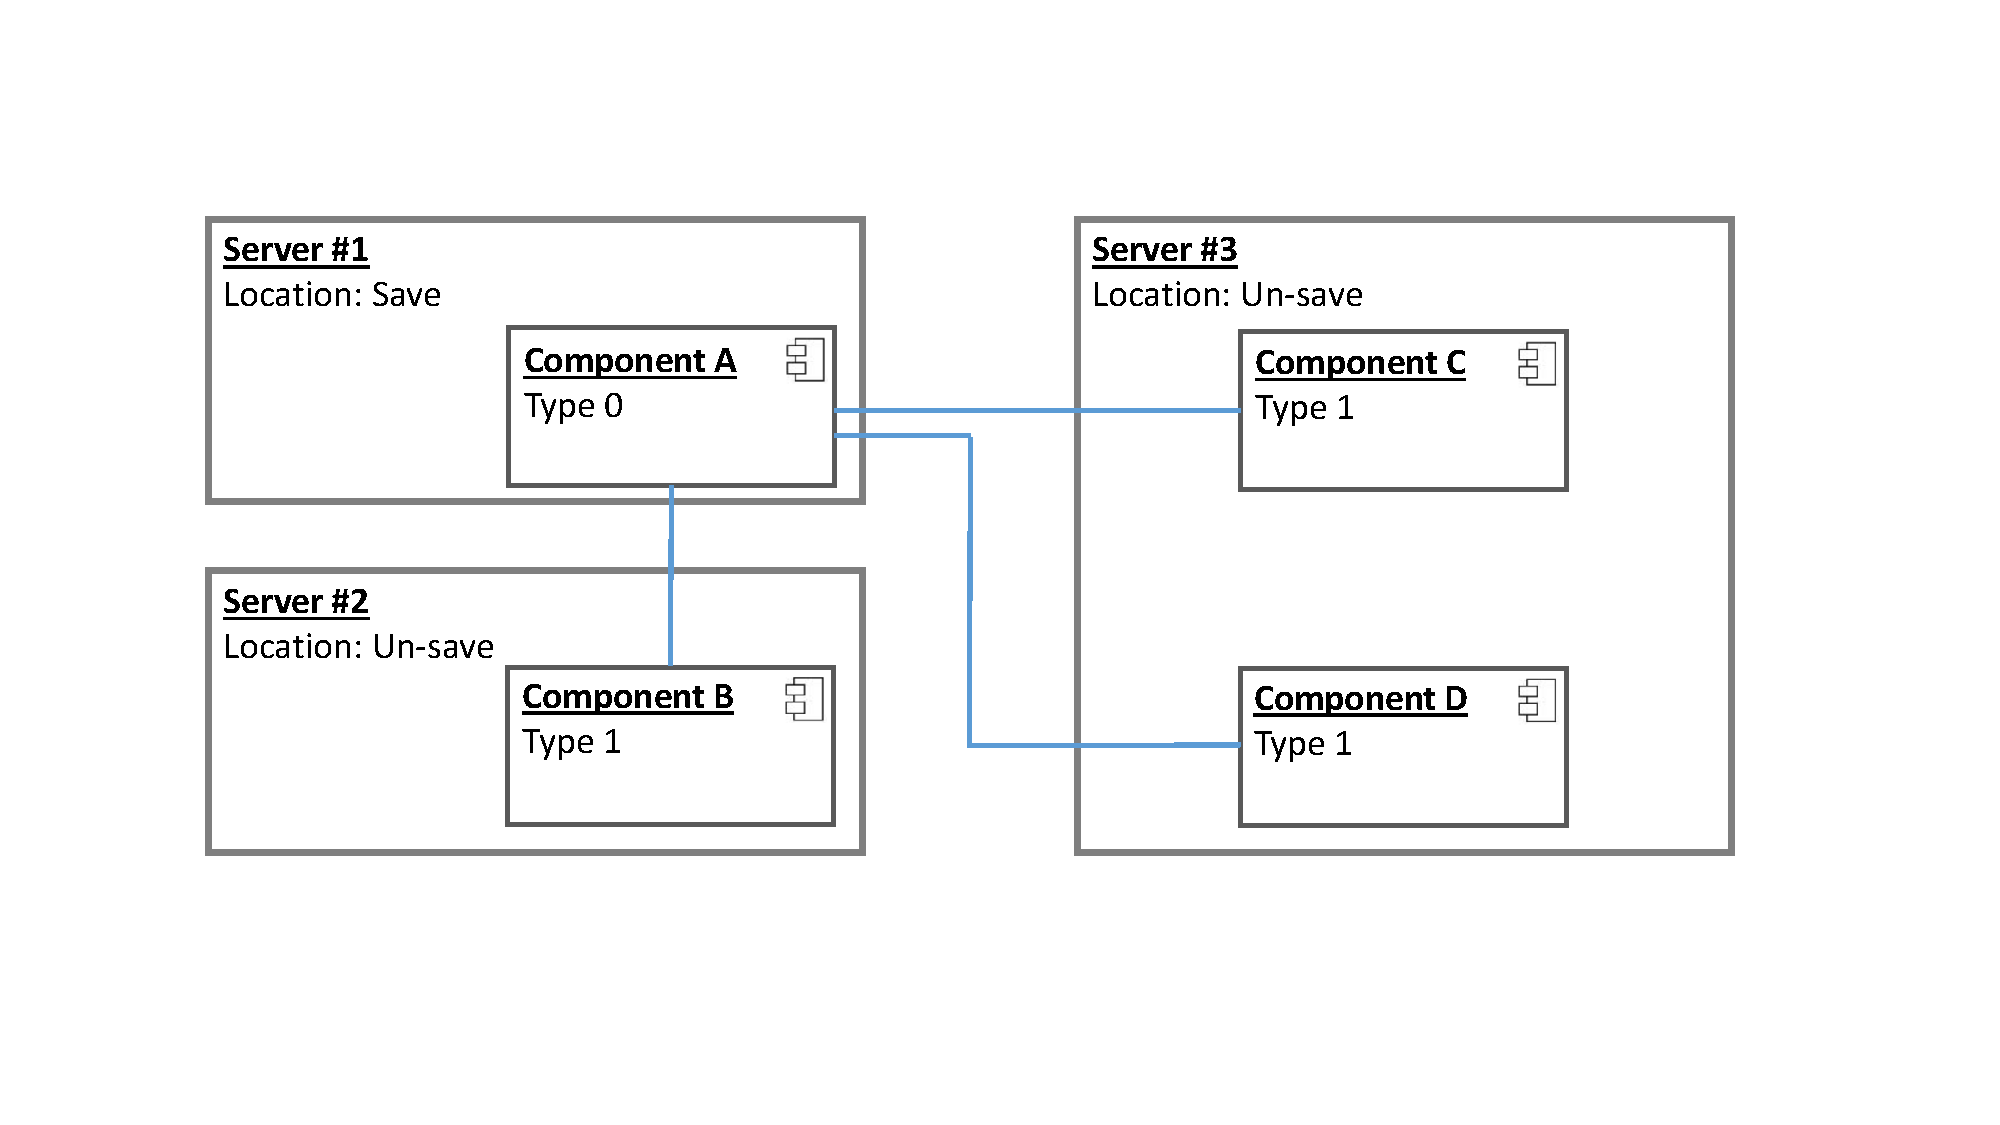
\includegraphics[trim = 35mm 45mm 40mm 30mm, clip, width=0.53\textwidth]{graphs/deployment_example_2}
	\end{center}
	\caption{Privacy violating deployment}
	\label{fig:example_depl:2}
\end{wrapfigure}

\textit{Rule 1 \& 2} don’t need any further explanation. \textit{Rule 3} states that Type 1 components can be deployed anywhere. This is due to the fact that Type 1 data should not contain any personal information. \textit{Rule 4} however limits this deployment. This constraint is necessary, because the combination of multiple Type 1 data streams could lead to privacy relevant information. If the data streams, however, have a common type 1 component as data source, the deployment can be considered privacy compliant. Note that data streams with type 2 components can be ignored, since - by definition - they don't get in contact with any privacy relevant data. \autoref{fig:example_depl:1}, \autoref{fig:example_depl:2} and \autoref{fig:example_depl:3} illustrate the different base scenarios applying to Rule 4. 

	
\begin{wrapfigure}{l}{0.55\textwidth}
	\begin{center}
		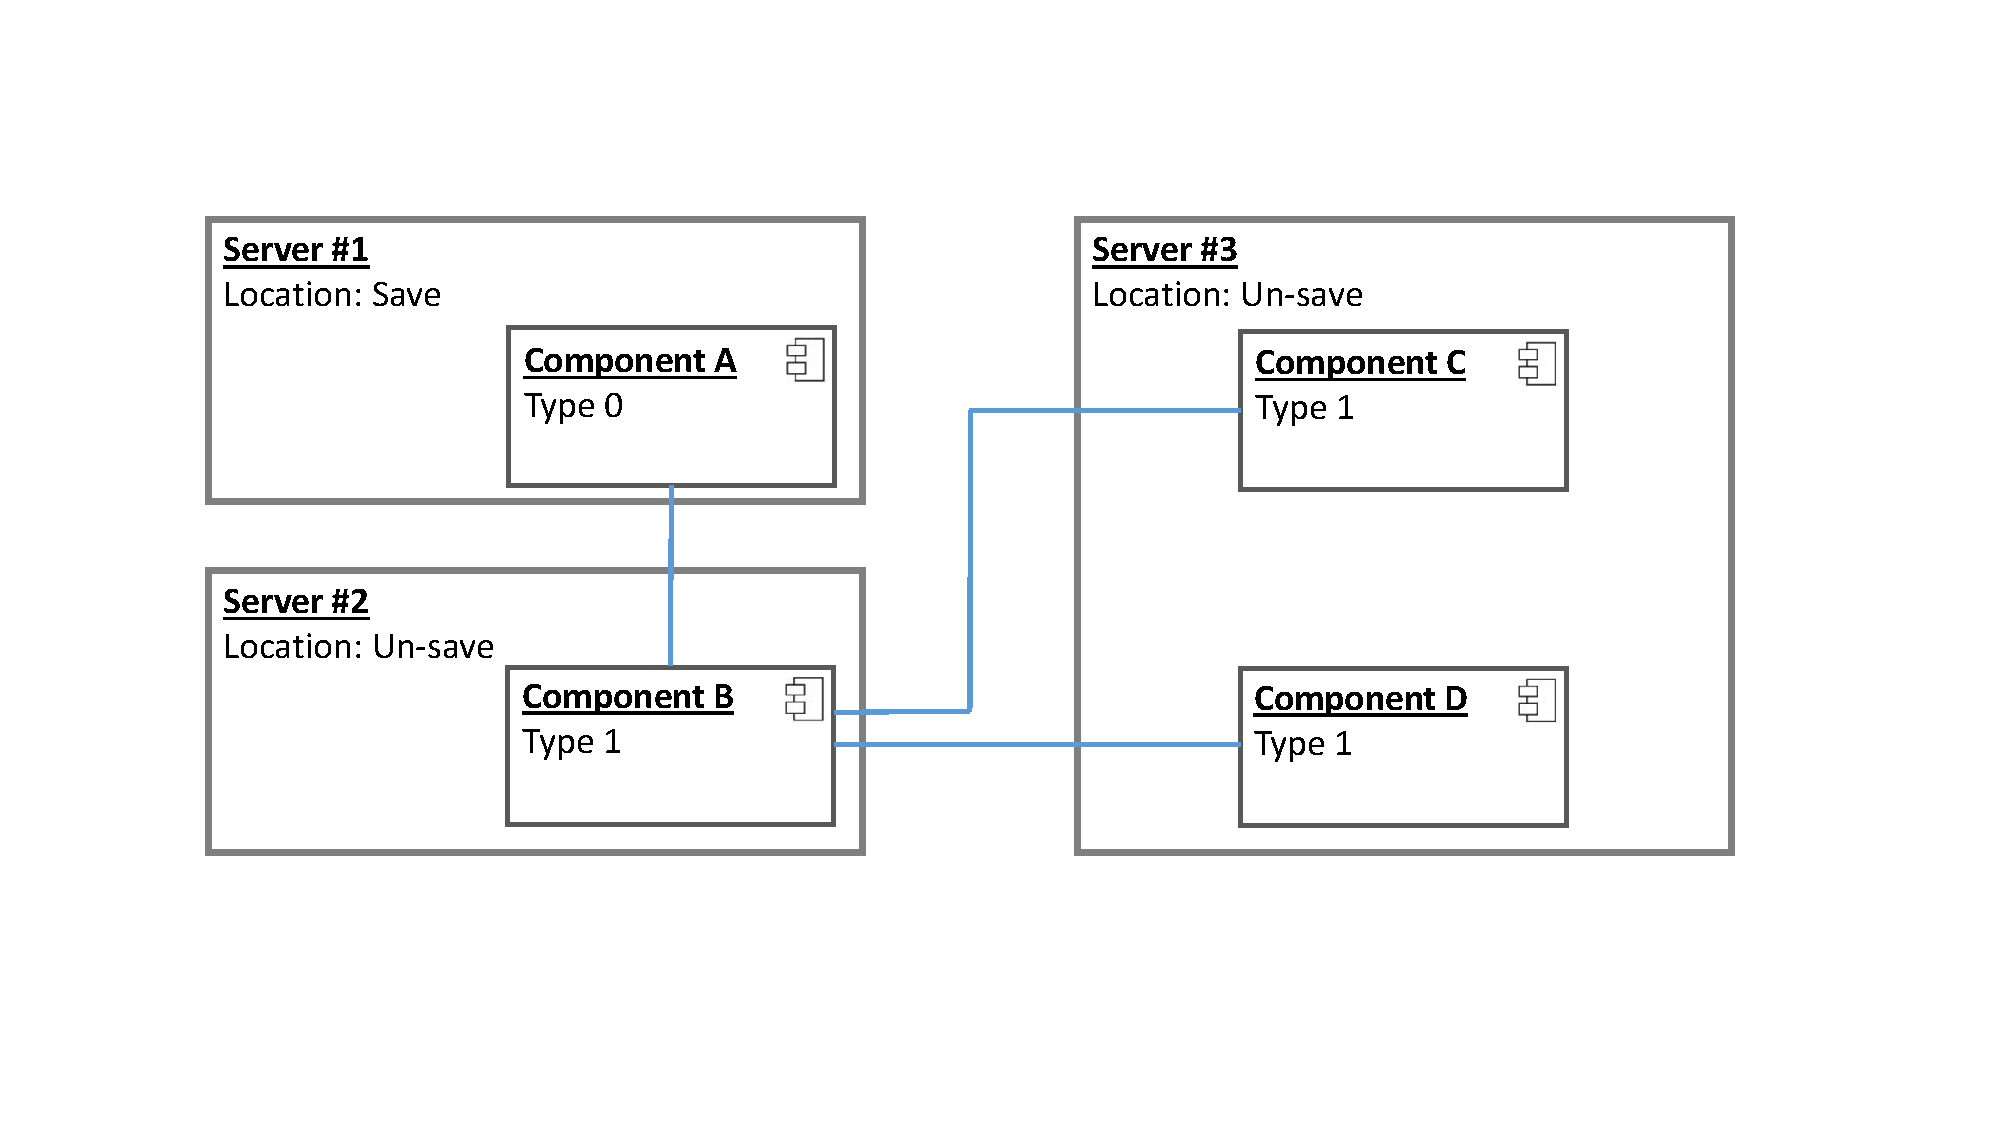
\includegraphics[trim = 35mm 45mm 40mm 35mm, clip, width=0.52\textwidth]{graphs/deployment_example_3}
	\end{center}
	\caption{Privacy compliant deployment}
	\label{fig:example_depl:3}
\end{wrapfigure}

The deployment shown in \autoref{fig:example_depl:1} is illegal. Server\#3 contains components with data streams from two different components, where one is a type 1 and one is a type 0 component. Even though they have a communication path, Component A could send different information to Component B and C. As a result, \textit{Server \#3} hosts two type 1 components, which don't contain privacy relevant data by themselves. However, after combining, could be privacy relevant. So, this deployment is illegal.

\autoref{fig:example_depl:2} also shows a illegal deployment. Component C and D share the same data source, which is marked as type 0. The same as before, the combination of data on Component C and D could lead to privacy relevant informations on \textit{Server \#3}.

The final example (\autoref{fig:example_depl:3}) is a legal deployment. This is because, Component C and D share the same data source (Component B), which already only contains type 1 data. This means, Component C and D can just contain data which are already available on Component B. This means, even through data combination and extensive data analysis, no privacy concerning information can be extracted.

We are aware, that these are over-approximations towards legal compliance. Nevertheless, we argue, that these simple, high-level rules already help to identify illegal deployments and establish privacy compliant (re-)deployments.


\section{Component categorization}
\label{sec:PrivacyConcept:comp_cat}

Components can be very complex due to multiple communication partners and dozens of interfaces. In such cases it can be considered impossible, to keep track of every single information flow on every component. This shows us, that a component - as a whole - shouldn't be categorized by hand.

But a single data stream between two component is easy to understand and easy to analyse. In an component based software architecture, data exchange happens via component interfaces. And during system composition the software architect must be aware of what data he passes through an interfaces.

As a result, we decided to categorize each interface communication during system composition. The components privacy categorization is then derived by evaluating the components communication.

We need to point out, that this categorization is only valid under the \textit{Closed World Assumption} (CWA) \cite{Sequeda.CWA}. Simplified, the CWA states, that if a system doesn't contain any information about a given statement, this statement is automatically wrong. Applied onto the privacy concept this means: The model contains all the information and information sources there are. Naturally, this assumption is wrong, since every component is connected to the internet and can access a nearly infinite amount of data. However, we need the CWA, in order to be able to make any statement about the systems privacy compliance. This is due to the high abstraction level - the system architecture - we have an information source.


\section{Information storage}
\label{sec:PrivacyConcept:pcm}

We are using the Palladio Component Model (\autoref{sec:Foundations:pcm}), which is just one of several Architecture Description Languages. Most ADLs share a comparable structure, which can differ, due to the designated purpose. We will describe the storage exemplarily on the PCM.

The runtime model is supposed to reflect every relevant information, concerning the models purpose. So, we need to store the components privacy level and the servers geo-location in the PCM model.

The geo-location belongs to a server, which is part of the resource environment model in PCM. The resource environment contains resource containers, which represents a server or virtual machine. So the resource container is the perfect place for storing the severs geo-location.

As mentioned in \autoref{sec:PrivacyConcept:comp_cat}, we need to categorize the communication between two connected component interfaces. The PCM system model uses the Assembly Connector to connect two component interfaces. This is the optimal model element to store the data privacy level for the inter interface communication.

%The PCM meta-model provides the repository model for component and interface specification. These are abstract and can be designed for multi-purpose usage. A database component for example can store any kind of data. This means a categorization during specification is not possible. This makes the repository model the wrong place to store the data privacy level. The system model represents the whole software system structure during runtime. This means, the purpose of a component and its neighbours are known and defined. This makes it ideal for data privacy marking.




%\todo{@Robert: Describe in view of a generic ADL or related to Palladio? CON ADL: To generic, could be anything! CON Palladio: Topic of Section PCM Extension}
%Since our base application iObserve uses the Palladio Component Model (\autoref{sec:Foundations:pcm}) we need to get the components data privacy type into the model. At first glance, this seems straight forward: Save the Data Privacy Level during design time as a components attribute. This however isn't a good solution, since the a components purpose is often not as clear as it seams. A database component for instance can contain personal, type 0 data or anonymous, type 2 data, pendent on its actual usage. As a consequence privacy levels should be applied during the system composition phase. In Palladio represented by the system model. This enables the system architect to classify two instances of the same component type differently.

%Components can be very complex, which usually results in a complicated and unintuitive data-flow. In such cases it can be considered impossible, to keep track of every data stream at once. This shows us, that a component as a whole shouldn't be categorized, but the "data-exchange points". These points are interfaces and represent the communication paths between components. While good interface designs share the same abstract multi-purpose intention as components - during design time. However, while composing the software system, it must be very clear to a software architect, what kind of data are transmitted between interfaces. In the PCM system model, provided interfaces and required interfaces are connected via an Assembly Connector. This is the optimal model element for categorizing the communicated data.